
\chapter{Static gestures recognition}

As was already mentioned, the detected gestures can be divided into two groups: static gestures and dynamic gestures.
The static gestures can be understood as a chosen position and orientation of the fingers and hand in a single moment, while dynamic gestures are defined as a movement of the hand and fingers in time. 
The problem of recognition of those gestures is a subject of following chapter. 
Firstly, the proposed approach is presented, followed by the introduction to the evaluation scheme. 
In last section, the performed experiments are descriebed, which were used to examine the effectiveness of proposed static gesture recognition approach.

\section{Proposed methods}

The static gesture recognition problem can be stated as a problem invariant to time.
That means that for each detected hand, the position and orientation can be treated as a new data uncorrelated to previously classified data.
While this assumption means that one can easily generate multiple samples from the sensors in short time, it also gives an opportunity to look at the static gesture recognition problem as a problem of classification.

While for most 2D gesture recognition problems simple classification algorithms seems to work well enough, the 3D data is more complication to model by the set of features and finally successfully label.
While dealing with 3D data, the position and orientation of hand can be easily affected by the height of the hand above the sensor or small change in the orientation of the hand with respect to the sensor's coordinate system. 
It is intuitively understood, that the system should recognize those gestures as the one as they are similar.
To meet those requirement, one need to define what is meant by the ,,small'' change in orientation resulting in treating the static gestures as the same.

\begin{figure}[htb]
\centering
 \includegraphics[width=0.6\columnwidth]{figures/SVM.png}
 \caption[]{SVM is a technique searching for the hiperplane that maximizes the margin between classes\footnotemark}
 \label{svmmargin}
\end{figure}



To meet those requirements, the Support Vector Machines \cite{Cortes:SVM} were used as a classification algorithm.
The SVMs were chosen as there exist a solid mathematical background supporting the simple idea of maximalizing the margin between classes.
Moreover, the SVMs were chosen also because of the popularity due to the open-source library libSVM \cite{libSVM}, which contains the multiple platform SVM implementation.
It is worth noticing that in original work, SVMs were used only to classify between two classes, but the idea was expanded to utilize the one-vs-all scheme allowing to classify multiple class sets.
The efficiency of SVMs depends on correctly choosing the kernel function used to map the separation problem into higher-dimension with expectation to achieve problem easier to solve.
The typical kernel functions:
\begin{itemize}
\item linear: $K(x_i, x_j) = x_i^Tx_j$.
\item polynomial: $K(x_i, x_j) = (\gamma x_i^Tx_j + r)^d, \gamma > 0$.
\item radial basis function (RBF): $K(x_i, x_j) = exp(-\gamma ||x_i - x_j||^2), \gamma > 0$.
\item sigmoid: $K(x_i, x_j) = tanh(\gamma x_i^Tx_j+r)$.
\end{itemize}
where $\gamma$, $r$, and $d$ are kernel parameters. According to the authors of the library, linear kernels should be used for linearly separable problems, while RBF kernel is the most versatile one.

\footnotetext{\url{http://en.wikipedia.org/wiki/File:Svm_max_sep_hyperplane_with_margin.png}}

The problem of classification assumes that each sample consists of set of features, which describe this sample and can be used to distinguish it from the other samples.
Additionally, each sample has a known or unknown label, which defined the membership of sample to the class. 
The samples with the known labels can be used to train the classification system to compute the membership to the classes for the samples. 
The computation is performed on previously mentioned sets of features.

In application of gesture recognition the classification be divided into two flows: the training part and the recognition part. 
In training part, the library will be provided with the samples of static gestures with known correspondences to the static gesture classes. 
From those samples, the sets of features are computed, which are used to train the classifier.
The recognition part assumes to have trained classifier. 
The recognition part is provided with samples static gestures without labels. 
For each sample the sets of features are computed and then given as input to the trained classifier.
The classifier returns the information of the gesture's class membership (label) of each sample.

In case of library, it is assumed that the learning process can be done offline, while strict online requirements has to be met in recognition part. 
To meet those requirements the Support Vector Machine is introduced[]. 
The SVM classification is commonly used technique in multiple areas of research as biology, robotics or IT for solving data classification problems [].
Additional advantage of the SVM is possibility to use C++ library libSVM[], which provides an easy interface to utilize this classification methods in different problems.

\begin{figure}[htb]
\centering
 \includegraphics[width=1\columnwidth]{figures/StaticGestures.png}
 \caption[]{Proposed solution blocks for learning and recognitnion parts of static gestures recognition problem}
 \label{svmmargin}
\end{figure}


While presented approach can be treated as state-of-the-art approach it still cannot be used without defining proper feature sets for gesture recognition.
The naive solution would be to use the raw data from Leap motion sensor as the feature set.
This solution was tested, but provided poor results as the proposed features were dependent on the position, orientation and scale of hand. 
Even small movement in any direction meant problems with stable recognition. 
The theoretical literature suggests to compute a set of features invariant to wanted transformations, which can allow to fully distinguish between different classes.
Unfortunately, there are not available propositions to feature sets when it comes to the gesture recognition using the data even similar to the data provided by the Leap Motion sensor.
Reminding, the Leap Motion for each frame allows to capture:

\begin{itemize}
\item position in X, Y, Z of each recognized finger
\item unit vector of each recognized finger
\item the width and height of each finger
\item the normal vector of the hand
\end{itemize}


\section{Evaluation methodology}

\subsection{Assumptions}
To provide user with library working in different conditions, it was assumed that the gesture is treated as the same one independently with respect to the translation, rotation and scale of the hand. 
This assumption means that the static gesture rotated by unknown angles, translated in sensor coordinate system and also with different hand sizes should still be recognized as the same gesture.
Invariance to the rotation, translation and scale poses a great challenge to the recognition, but allows the future users of API to fully utilize the feasibility of the library.
It is worth mentioning that, it does not reduce the possible applications of the library, as an assignment of static gesture to already defined class allows to find the transformation between the model of the class and observed gesture.


\section{Recorded datasets}

To propose and test the quality of the features twelve static gestures were chosen:
\begin{enumerate}
\item the peace sign,
\item a fist,
\item full hand with space between each finger,
\item American Sign Language: ``I love you'' sign,
\item sign ``gun'' created by putting thumb and forefinger up, while holding the rest fingers in a fist,
\item all fingers in a fist with exception of thumb, which is up,
\item the sign X made with the forefingers of both hands,
\item the sing ``Time'' used e.g. by coaches in basketball games.
\item sign simulating rotating a knob by two fingers,
\item sign simulating rotating a knob by five fingers.
\end{enumerate} 
The gestures are also presented at fig.~\ref{staticgestures}.

\begin{figure}[htb]
\centering
 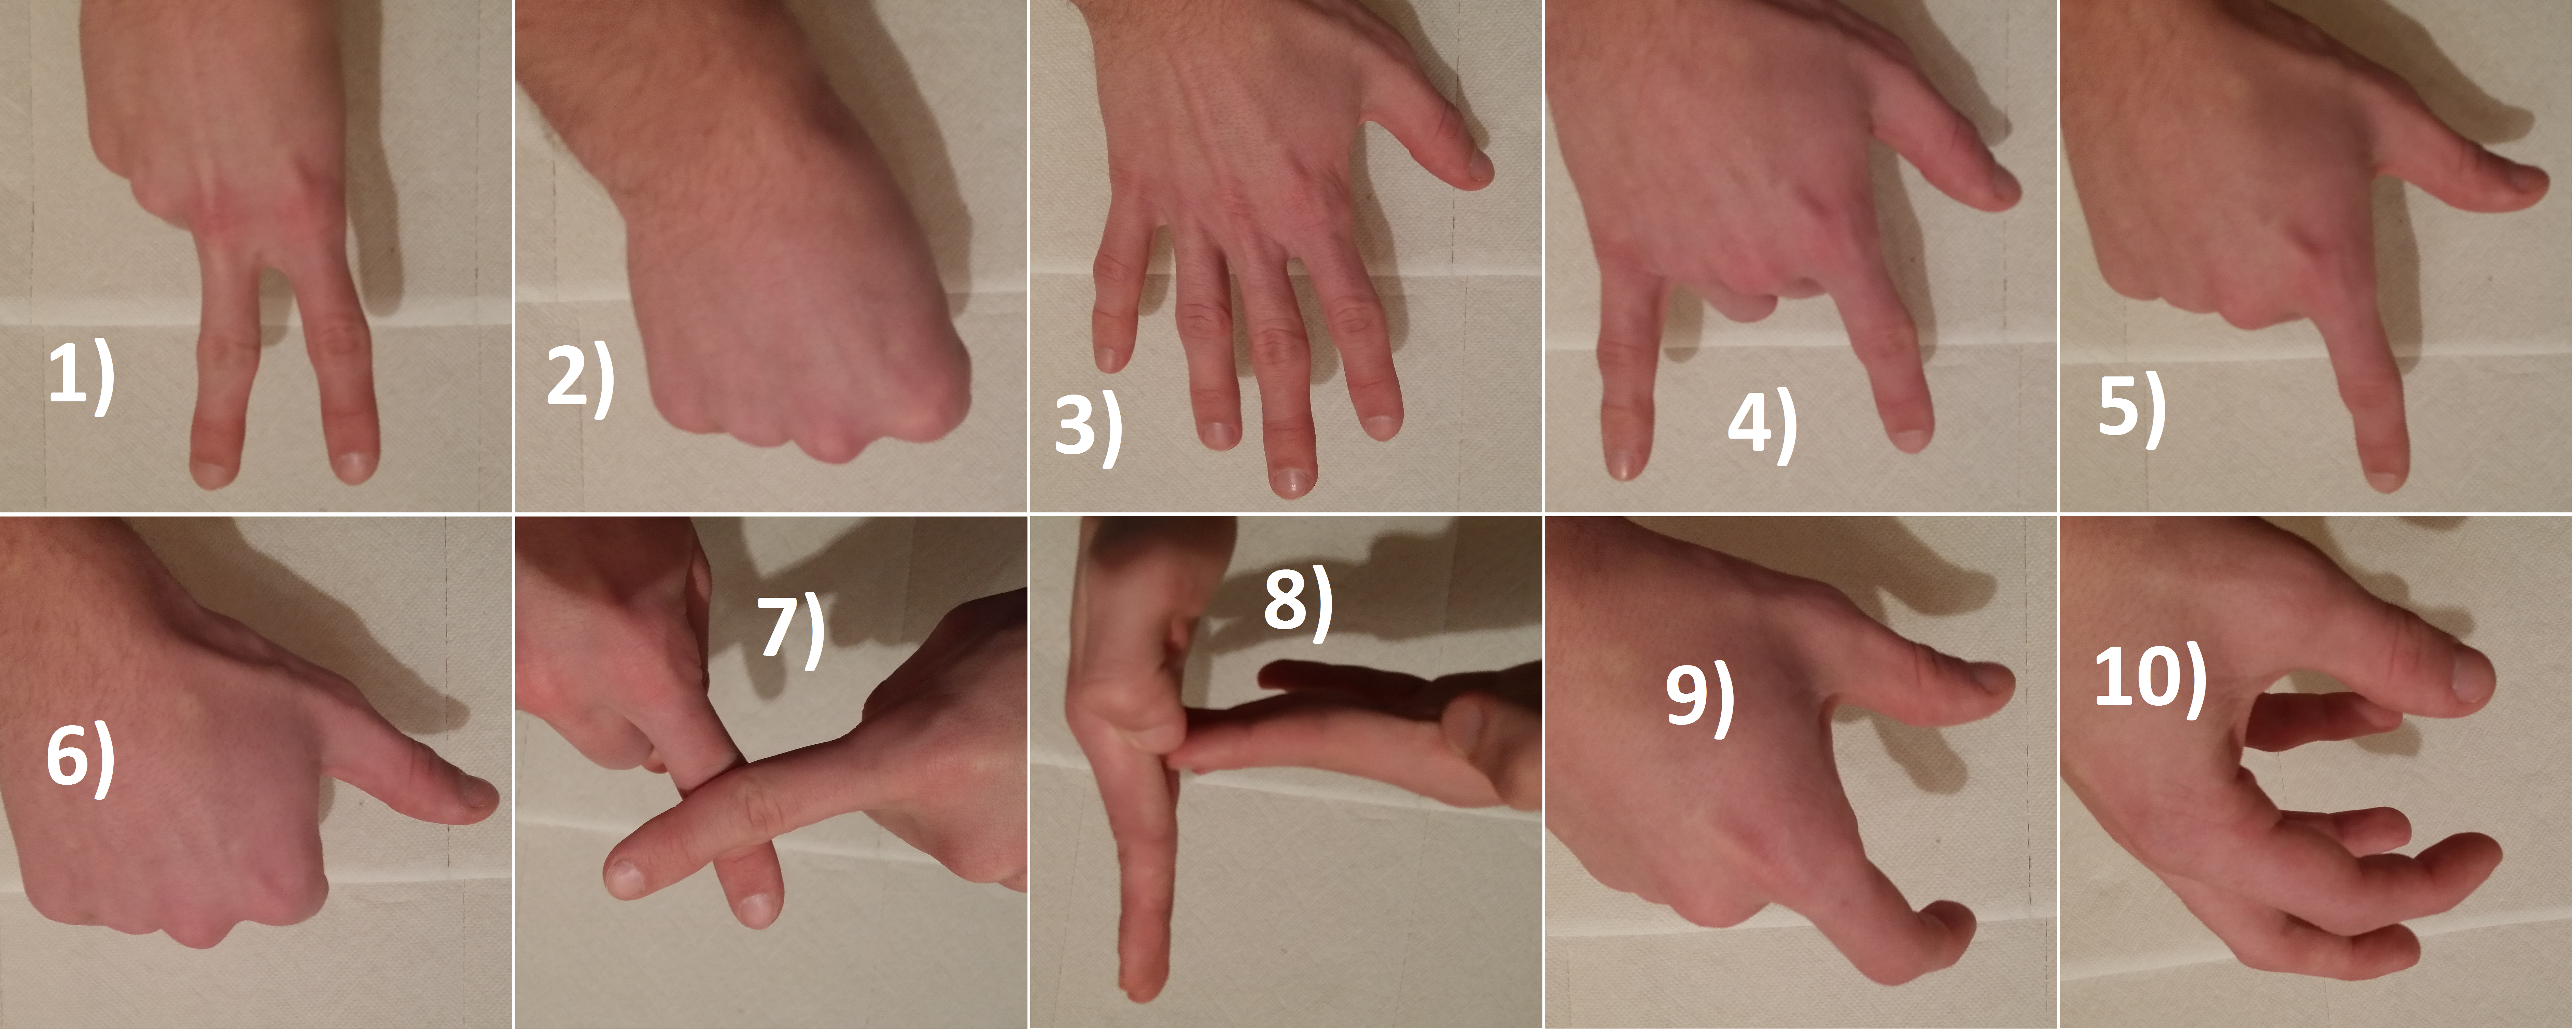
\includegraphics[width=1.0\columnwidth]{figures/static_gestures.png}
 \caption{Figures chosen for the comparison of different classification approaches}
 \label{staticgestures}
\end{figure}

The sample data of each gestures were recorded using the continuous mode of recording, while moving the hands in different directions and changing the orientation of the hands. 
For each of the proposed gestures, each author recorded approximately 1000 samples.

Having samples with known labels, the whole dataset was separated into training and testing sets in relation 2:1. 
For the training, the k-fold cross-validation (CV) scheme was used, which searches for optimal $C$ and $\gamma$ parameters trying to prevent the algorithm from over-fitting the training data.
This method is used to find the optimal parameters of the classification system, while estimating the performance on the data not used in the training part. 
In standard version of the method, the gathered data is divided into two sets: one containing k-1 parts of the data, the other 1 part of the data. 
The first is used to train the classification system, while the rest of the gathered data is used to estimate the performance. 
The performance is estimated by calculating the number of cases when the classification system returned a label which matched already known label. 
The percent of correctly recognized labels to the total size of the testing set is known as recognition rate.



The first proposed vector of features consisted of:
\begin{itemize}
\item number of fingers in frame,
\item the absolute angles between fingers and the normal of the hand,
\item the absolute angles between consecutive fingers,
\item the euclidean distance between consecutive finger's tips.
\end{itemize} 

After approach allowed to achieve XXX\% of recognition rate and was unsatisfying from the perspective of feature application. 
Analysis of the finger numbering revealed that the fingers are numbered accordingly to the position in Z axis of the tip of the finger.
This means that when features are approximately on the same position in Z axis, the numbering can change rapidly and proposed features compare different fingers.
To achieve the features that would be invariant to the numbering of the fingers, the feature set was changed.
Instead of containing the absolute angles and distances between consecutive fingers, it was proposed to contain the five greatest values of angles and five greatest values of distances between all combinations of finger pairings.
This approach was tested on the same training set and allowed to increase the recognition rate to the 83.8812\%.
While the number of fingers in frame and five greatest angles between all possible angles between fingers are invariant to the translation, rotation and scale, the distances between tip position were dependent on the scale of hand.
To achieve distances invariant to the scale of hand, it was proposed to exchange the five greatest distances for five greatest ratios of the distances between tips of all fingers to the maximal found distance between tips of all fingers.
As this approach was expected to increase the recognition rate, it fell down to 77.0913\%.
More experiments with enlarging the set of features to having ten greatest angles and ten greatest distances showed slight fall in recognition rate to 83.7687\%. 
The all results have been presented in table [].

To increase the recognition rate an attempt to gather more training data was performed, which end with recognition rate equal to XX\%. 
While using more data, it is worth noticing the growth of training time. In case of 5000 samples the typical training process took approximately 6 hours. 
This computing time can be unacceptable by the users of the library, so the test with another SVM library libLinear[] was performed. 
The libLinear's implementation of SVM utilizes the linear kernels, which are useful for large data training sets with multiple number of features. 
This library reduced the training time to about 20 seconds, but the best obtained recognition rate was 64.524\% for libLinear compared to the 83.8812\% for the libSVM.


The firstly tested set of static gestures contained gestures, which were did not take into account the way how the Leap Motion works and for gestures like fist or 'X' the recorded data contained almost no information how to classify those gestures.
That's why the experiments were repeated on the five gestures, which could be easily distinguishable by data provided by Leap Motion. To this experiment the gestures peace, hand, ''I love you'', fist with thump up and rotating knob by 5 fingers were chosen.
For this classification problem with feature set defined by number of fingers, 5 greatest absolute angles and 5 greatest absolute distances between fingers, the recognition rate of 90.9532\% was achieved. 

The last test performed for static gestures recognition consisted of classifying the set of 10 possible static gestures. For this test the recognition rate of 73.2118\% was achieved.

